\section*{Introduction}
In particle detection one of the first and most important requirements is the production of a time reference for detected events. Correct definition of a particle detection time  is essential to allow the production of coincidence signals between the different detectors which compose the arrays of an experimental set-up. Moreover the reduction of timing error  is crucial for several measurements, such as the \textit{Time of Flight} (TOF) technique, used to distinguish the particle type but also to measure its kinetic energy.

There are several ways to produce a timing reference for detected particles, the aim of a good technique is to increase the accuracy and reduce the dependence on particle energy (\textit{Time walk}).
The simplest one is the \textit{Leading Edge} method, which associates the time reference of the signal with the crossing moment of a fixed threshold, for instance 0.2 as shown in Fig.~\ref{fig:LE-CFD}-a. In scintillation detectors, where the rising time of the pulses is constant, this method is clearly affected by the amplitude of the signals, making it not good for the purpose. 
A better solution is the \textit{Constant Fraction Discrimination} (CFD) technique (Fig.~\ref{fig:LE-CFD}-b), which gives a time reference independent on pulse amplitude.
\begin{figure}[h!]
	\centering
	\subfloat[][\emph{Leading Edge method.}]
	{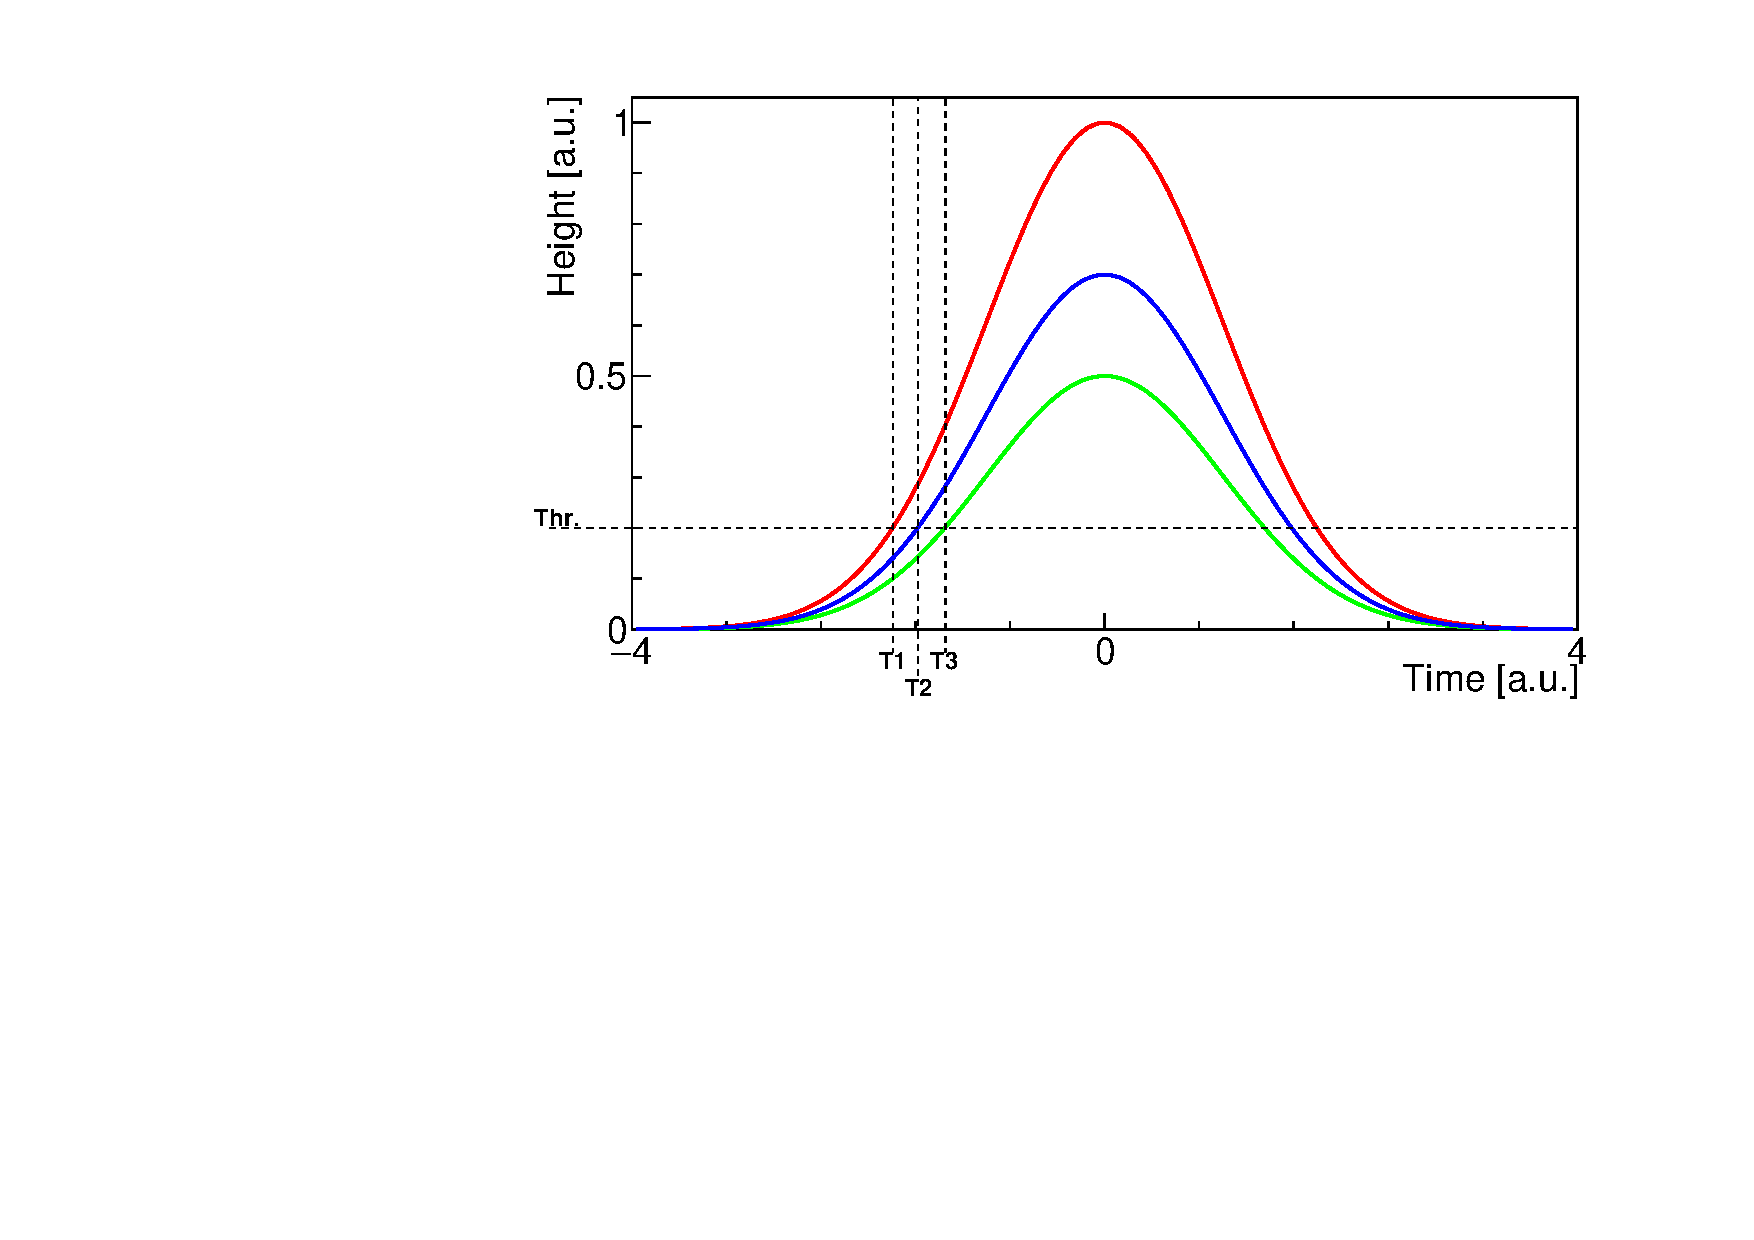
\includegraphics[width=.48\textwidth]{immagini/gausledge.pdf}} \quad
	\subfloat[][\emph{CFD method.}]
	{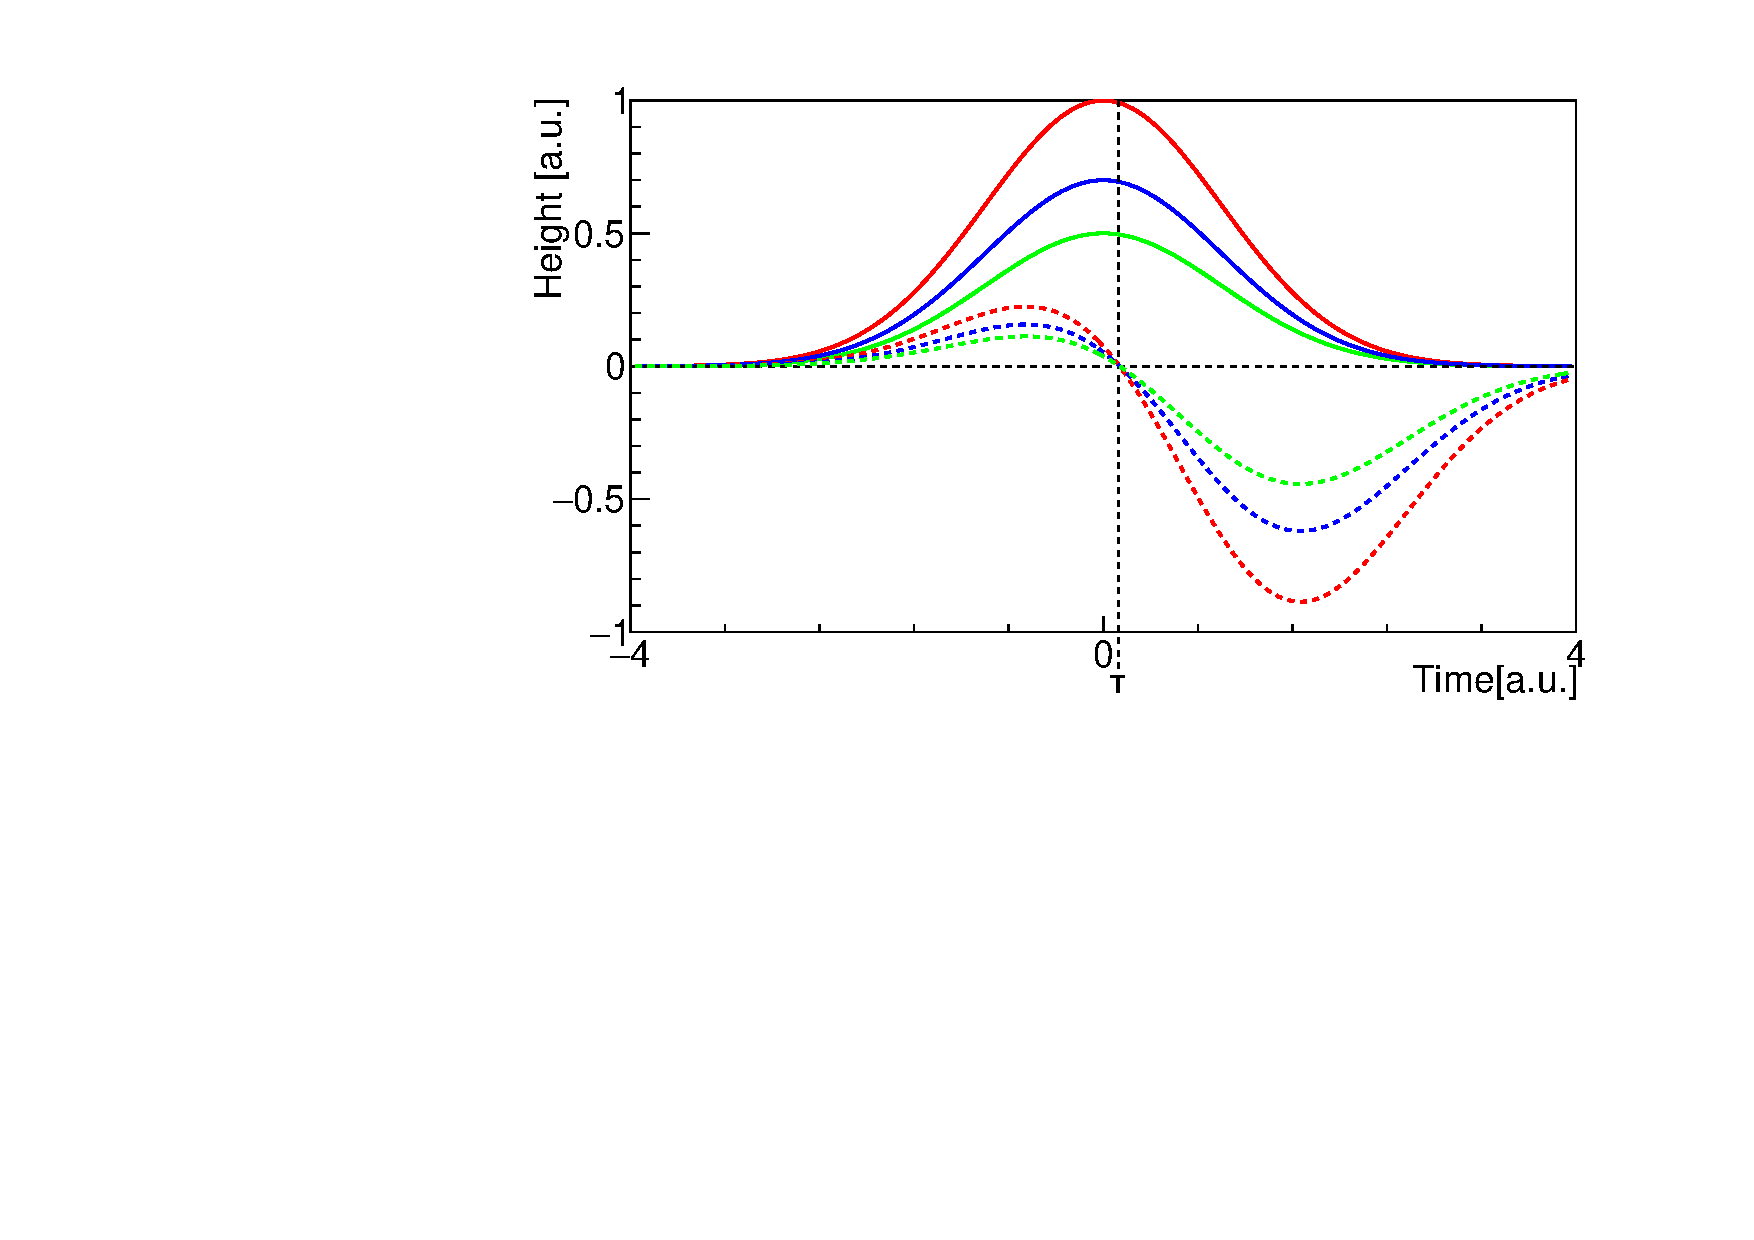
\includegraphics[width=.48\textwidth]{immagini/gauscfd.pdf}} \\
	\caption{\textit{Leading Edge} (a) and \textit{Constant Fraction Discrimination} (CFD) (b) techniques applied on three Gaussian pulses with same mean and sigma but different amplitudes. The bipolar dashed pulses in b) are generated by the CFD algorithm.}
	\label{fig:LE-CFD}
\end{figure}

The aim of this report is to present the timing analysis performed over two scintillation detectors. Therefore the  following sections will analyze these steps:
\begin{itemize}
\item Energy calibration of the organic scintillators and
calculation of the energy resolution from the analysis of
the Compton edge.
\item Optimization of the external delay of the analogue
CFTD to obtain the best time resolution.
\item Study the time resolution behaviour as a function of the
energy.
\item Comparison between the timing resolutions obtained
from analogue and digital treatment of the signals.
\item Measurement of the speed of light. 
\end{itemize}

\begin{figure}[h!]
	\centering
	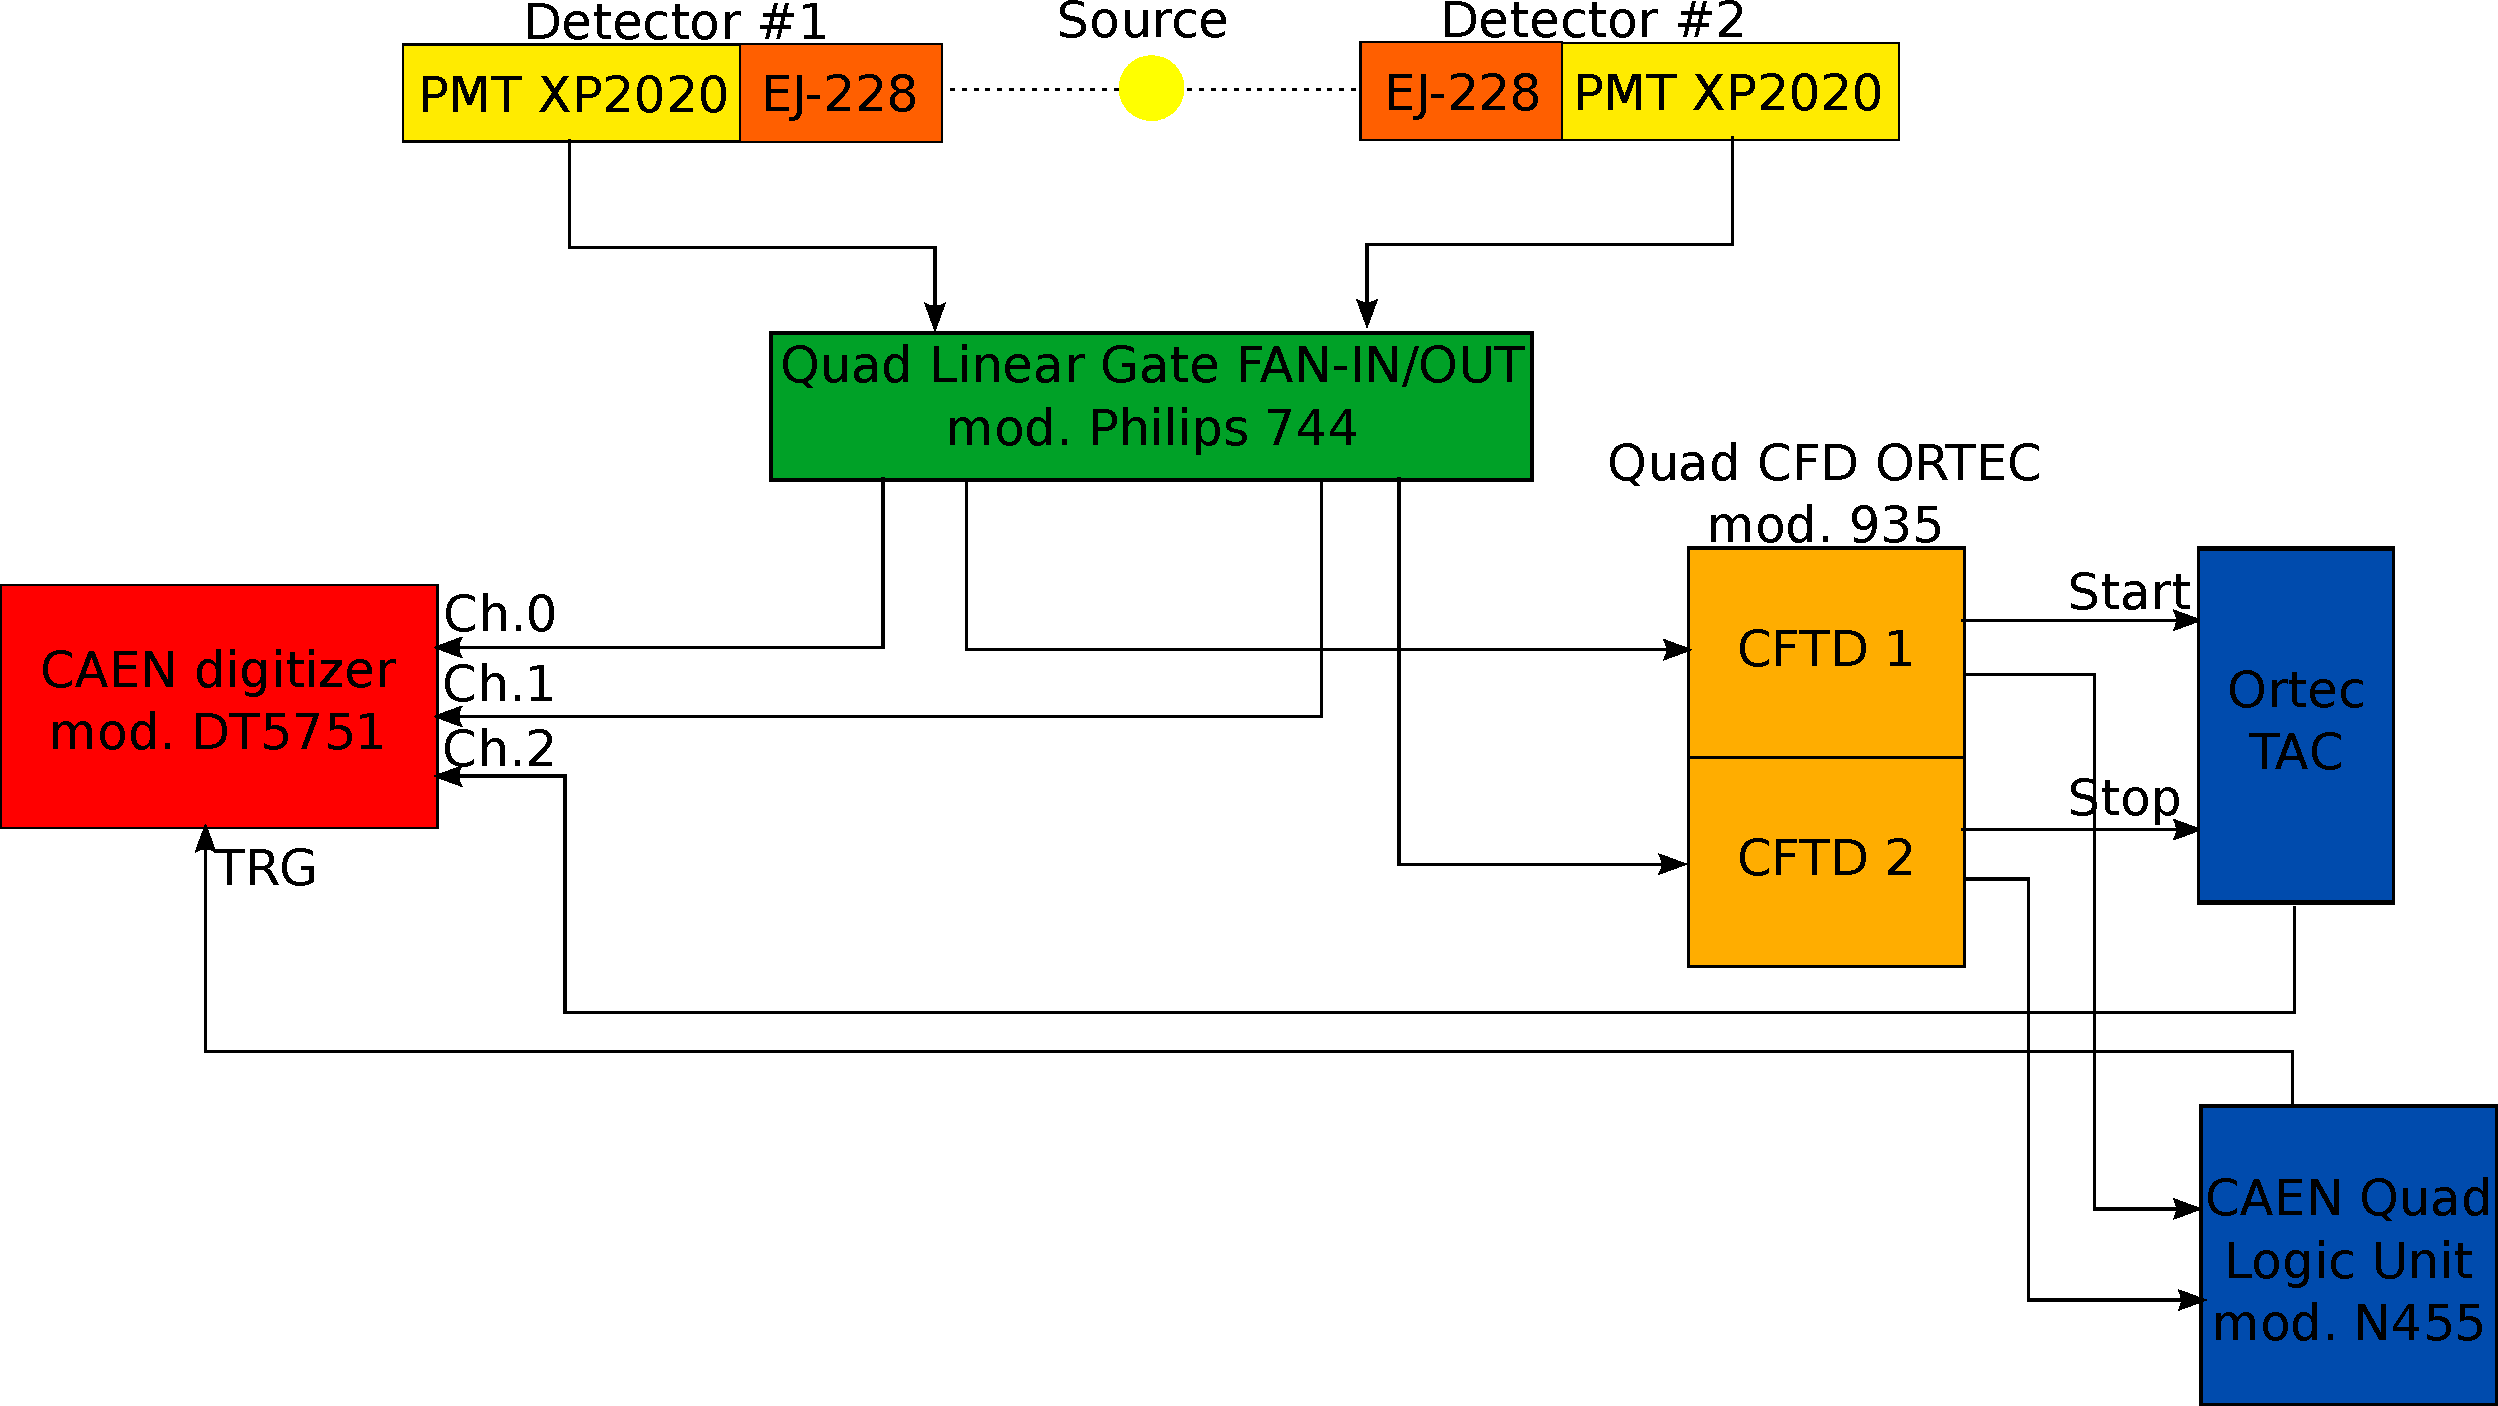
\includegraphics[width=\textwidth]{immagini/SetUp.pdf}
	\caption{Experimental configuration used in the timing analysis.}
	\label{fig:Set_up}
\end{figure}